\subsection{Introduzione a Gnome Desktop}

Nei sistemi operativi GNU/Linux esistono un gran numero di interfacce grafiche, differenti per caratteristiche e per destinazione d'uso. Alcune ad esempio sono pensate per essere più gradevoli e facili da utilizzare, altre per minimizzare il consumo delle risorse hardware. In molti casi, le distribuzioni Linux, siano esse di tipo "enterprise" o meno, offrono una selezione di queste interfacce per venire incontro alle esigenze dell'utenza. Senza nulla togliere alle altre, in questo testo faremo riferimento, parlando di interfaccia grafica, a quella nota come Gnome Desktop (predefinita in molti prodotti quali Red Hat, CentOS e Fedora). Gnome Desktop, deriva dal progetto GNOME (G.nu N.etwork O.bject M.odel E.nvironment), nato nel 1997 come alternativa al già affermato KDE, con l'idea di fornire \textit{"un ambiente grafico intuitivo ed invitante"}. Nonostante lo sviluppo costante abbia portato le versioni Gnome 3.X a dei buoni livelli di stabilità, in questo testo si fara riferimento alla versione 2.28.X.

\begin{figure}[!ht]
 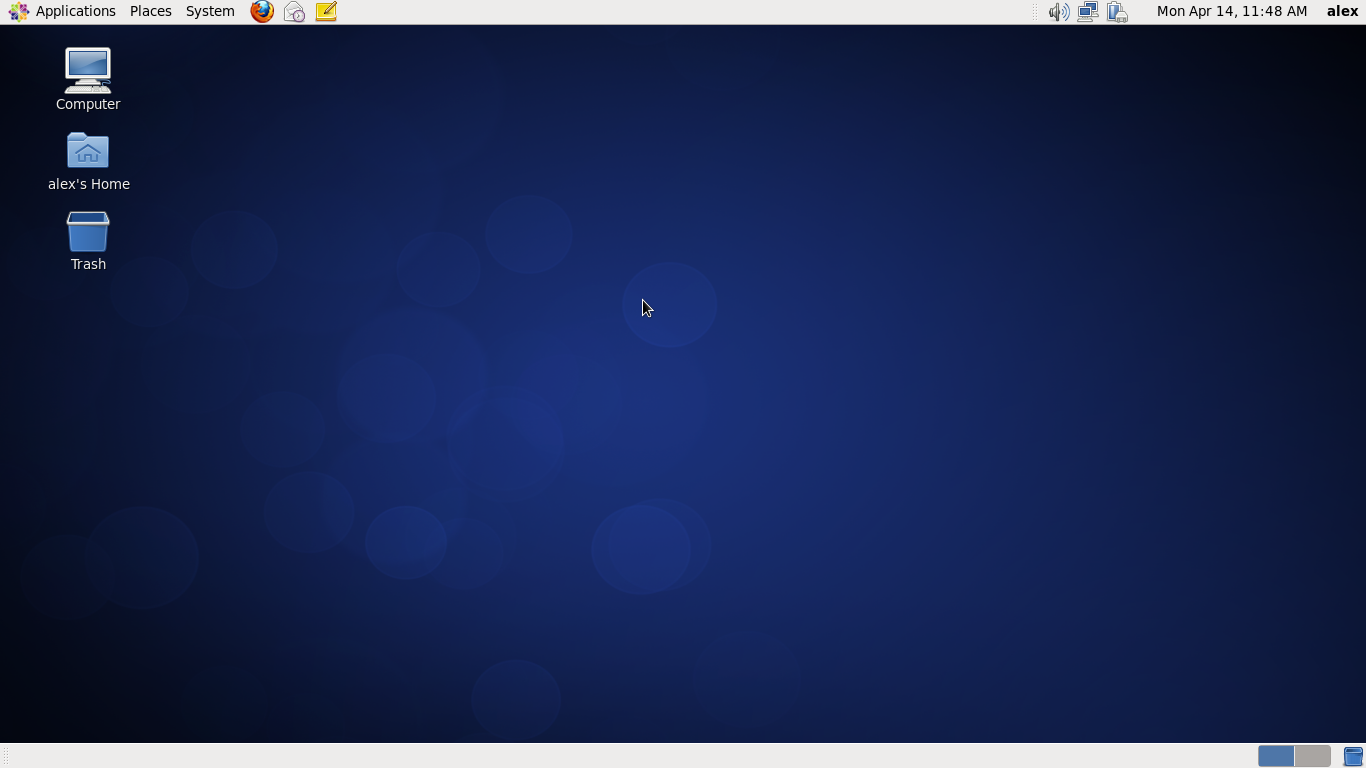
\includegraphics[scale=.24]{Immagini/UI_01.png}
 \label{fig:Gnome Desktop 2.28.2}
 \caption{Screenshot di GNOME Desktop 2.28.2 su CentOS 6.5}
\end{figure}

All'interno dell'interfaccia sono riconoscibili 3 elementi principali

\begin{itemize}
 \item panel
 \item applet
 \item workspace
\end{itemize}

\subsubsection{Panel}
Sono quelle barre, solitamente di colore grigio, presenti agli estremi dello spazio desktop. La dimensione ed il numero di questi pannelli è personalizzabile, così come il colore ed il contenuto. Nella configurazione in esempio troviamo un pannello sul bordo superiore ed inferiore del desktop. L'uso tipo è quello di contenere le applet o applicazioni speciali.
\subsubsection{Applet}
Normalmente sono visualizzabili come icone disposte sopra i vari panel. La loro funzione è variabile, e può fungere da launcher di applicazioni, così come essere un modulo di controllo per un servizio di sistema (es nm-applet di NetworkManager) o dei controlli del desktop (es. Workspace switcher)
\begin{figure}[!ht]
\centering
 
\includegraphics{Immagini/UI_Panel1.png}
 \label{fig:Panel Gnome}
 \caption{Alcune applet sulla pozione di un panel}
\end{figure}


\subsubsection{Workspace}
Si tratta dell'area di lavoro, all'interno delle quali, il gestore delle finestre posiziona le applicazioni che vengono aperte. All'interno è possibile trovare anche icone realtive ad alcuni percorsi di sistema e launcher di singole applicazioni. Differentemente da numerosi prodotti simili, Gnome offre Workspace multipli, dove è possibile collocare finestre differenti per ognun workspace. Lo switch tra i vari Workspace è ottenuto tramite la combinazione di tasti

\begin{itemize}
 \item \keys{CTRL + ALT + \arrowkeyleft }: Sposta sul workspace a sinistra
 \item \keys{CTRL + ALT + \arrowkeyright}: Sposta sul workspace a destra
\end{itemize}



%\begin{verbatim}
% [CTRL] + [ALT] + [LeftArrow]
%\end{verbatim}
%\begin{verbatim}
% [CTRL] + [ALT] + [RightArrow]
%\end{verbatim}

Esiste inolte una applet che visualizza i workspace e consente di eseguire lo switch tra di essi, che prende il nome di Workspace Switcher.

\begin{figure}[!ht]
\centering
 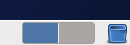
\includegraphics{Immagini/UI_WS_Switch1.png}
 \label{fig:Workspace Switcher}
 \caption{Workspace Switcher}
\end{figure}

\subsection{Applicazioni}

\subsubsection{Nautilus}

\begin{figure}[!ht]
\centering
 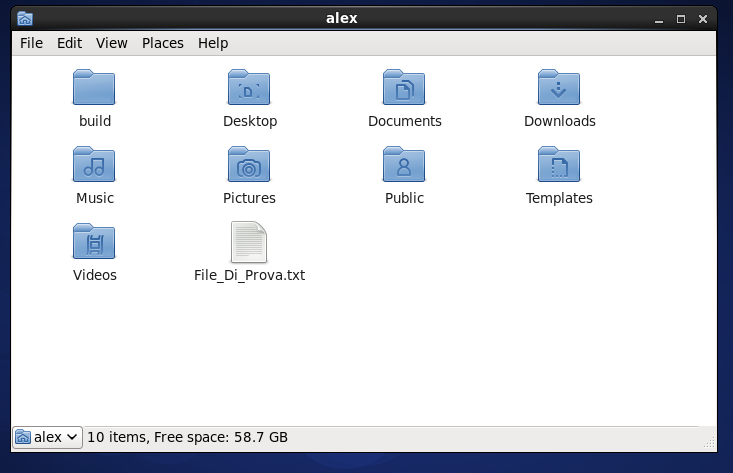
\includegraphics[scale=0.60]{Immagini/Nautilus1.png}
 \label{fig:Nautilus}
 \caption{Nautilus}
\end{figure}

\textbf{Nautilus} è un software della categoria File Manager molto potente e versatile; consente di poter consultare il contenuto delle cartelle con una intefaccia a fineste con viste configurabili. Per coloro che provengono da ambienti Microsoft\textregistered, possiamo dire che Nautilus è l'omologo Gnome del software Explorer.

Attraverso il menu \textbf{"View"} di nautilus è  infatti possibile definere la visualizzazione di file e cartelle con delle icone o con una lista organizzata. 
All'interno della lista è inoltre selezionare un criterio secondo il quale ordinare i file per ordine crescente e decrescente (es Data, Dimensione, Tipo, Nome). Inolte, con l'opzione \textbf{"Show Hidden Files"} si possono visualizzare i file marcati come "nascosti"; si tratta di file e cartelle il cui nomefile comincia con il carattere ".", ciò per impedirne la visualizzazione a meno che non sia espressamente richiesta. 

Nautilus consente di visualizzare percorsi locali (dischi interni, media rimuovibili e simili) e di percorsi remoti; attraverso la funzione \textbf{"Connect to Server"} è possibile collegarsi a macchine remote e sfruttare i file remoti come se fossero locali. I protocolli supportati sono:

\begin{itemize}
 \item Public FTP
 \item FTP Classic
 \item SSH (sftp)
 \item Windows Share (SAMBA, CIFS)
 \item NFS
 \item WebDAV
\end{itemize}

\begin{figure}[!ht]
 \centering
 \begin{subfigure}{0.4\textwidth}
  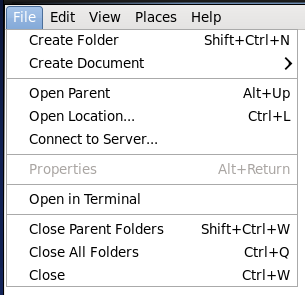
\includegraphics[scale=0.5]{Immagini/Nautilus_File2.png}
  \label{fig:Nautilus_File}
 \end{subfigure}
 \begin{subfigure}{0.4\textwidth}
  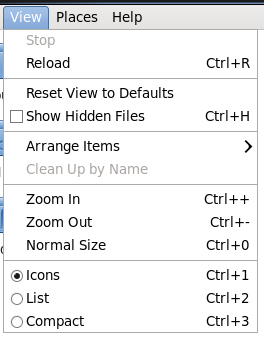
\includegraphics[scale=0.5]{Immagini/Nautilus_View2.png}
  \label{fig:Nautilus_View}
 \end{subfigure}
 \caption{Menù di Nautilus}
\end{figure}




\subsubsection{gedit text editor}

\begin{figure}[!ht]
 \centering
 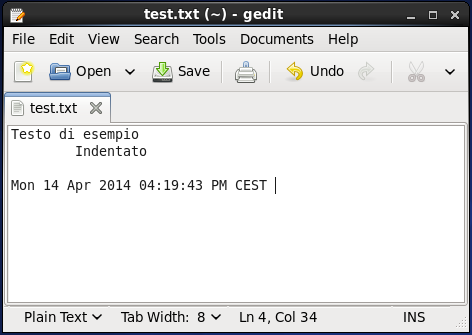
\includegraphics[scale=0.6]{Immagini/gedit1.png}
 \label{fig:gedit}
 \caption{gedit text editor}
\end{figure}


L'editor di testi \textbf{"gedit"}, è una applicazione atta alla lettura e modifica di file di testo semplici. A differenza del ben più noto omologo in ambiente Microsoft\textregistered (notepad), gedit dispone già di alcune funzioni avanzate. Ad esempio, dispone della funziona nota come \textit{"highlighting"} del codice per un gran numero di linguaggi di programmazione.

Gedit è reperibile nel menù alla voce \menu{Application > Accessories > gedit Text Editor}

\subsection{Guida in linea}

\begin{figure}[!ht]
  \centering
  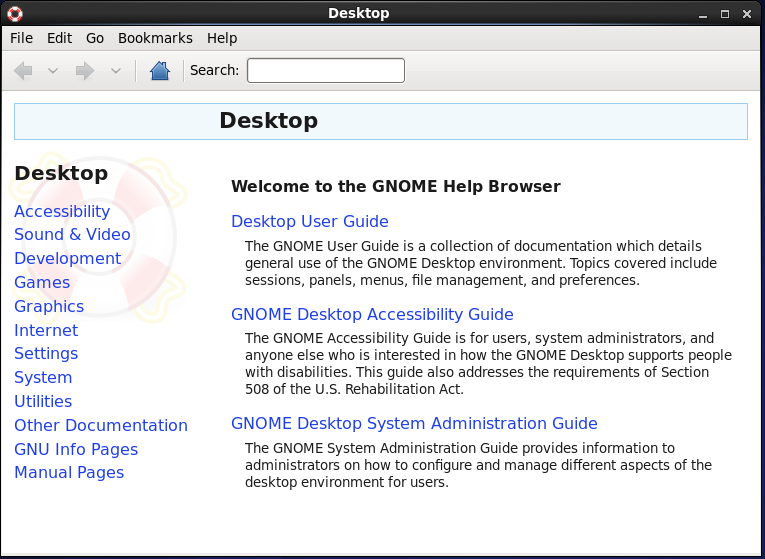
\includegraphics[scale=0.54]{Immagini/gnome_help1.png}
  \label{fig:gnome_help}
  \caption{Gnome Help}
\end{figure}

Dall'interfaccia principale di Gnome, premendo il tasto \textbf{[F1]} è possibile accedere alla guida in linea (oppure andando sul menù, selezionando la voce \menu{System > Help}. La guida è suddivisa in tre sezioni principali

% \textbf{System} $\rightarrow$ \textbf{Help})
\begin{itemize}
 \item Desktop User Guide
 \subitem Guida all'uso delle applicazioni utente, e dell'intefaccia.
 \item Accessibility Guide
 \subitem Guida per utenti ed amministratori interessati a scoprire come Gnone supporti le persone disabili nell'uso del sistema. 
 \item Administration Guide
 \subitem Guida agli strumenti di amministazione del sistema
\end{itemize}

Nel menù a sinistra è inoltre possibile consultare la guida suddivisa con il medesimo criterio di presentazione del menu delle applicazioni. 

